%mainfile: rapport.tex

\section{Identification unique des véhicules}
\label{section:vin}

En marge de l'implémentation des algorithmes de \pie, nous nous sommes interrogés sur les problématiques de sécurité liées à un tel type d'application.

Pour s'assurer du bon fonctionnement de l'algorithme, il faut qu'il y ait unicité de l'identifiant des émetteurs/récepteurs. En effet, comment acheminer des messages vers le bon destinataire si deux identifiants identiques existent?

La gestion des identifiants est donc cruciale, car en cas de manque de robustesse dans le choix de ceux-ci, il y des risques avérés de dysfonctionnement.
Réaliser un système de création d'identifiant centralisé serait contraire à la philosophie de fonctionnement de \pie, à savoir décentralisé les échanges de messages.

De plus, s'appuyer sur le pseudonyme des utilisateurs n'est pas suffisant : deux utilisateurs peuvent avoir le même pseudonyme. Comme nous ne pouvons pas imposer une unicité des pseudonymes d'utilisateur, il faut considérer une combinaison identifiant du véhicule / pseudonyme de l'utilisateur.

\subsection{\vinfull}
L'industrie automobile s'est penché sur la problématique de l'uniformisation de la numérotation de série des véhicules entre les différents constructeurs. La SAE (\etranger{Society of Automotive Engineers}) a donc introduit un mode de numérotation s'appelant \vin{} pour \vinfull.

Cette numérotation standardisée est définie par la norme ISO~3779.

Ce numéro comporte dix-sept digits et contient, en plus du numéro de série du véhicule, un certain nombre d'informations sur ses équipements.

Le numéro est constitué comme suit :
\begin{center}
	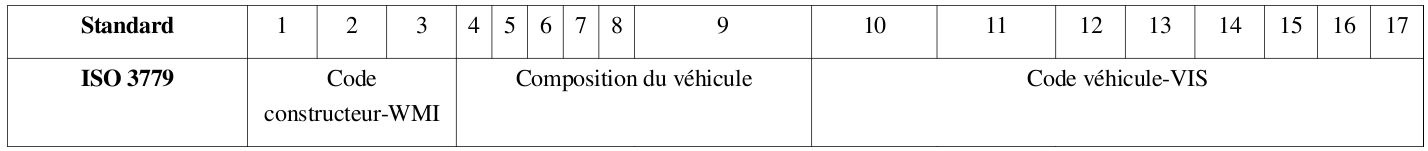
\includegraphics[width=0.9\textwidth]{img/vin}
\end{center}
Ce qu'il faut retenir est que ce système de numérotation fonctionne un peu comme le système de numérotation de l'adressage MAC dans le contexte des réseaux informatiques.

La première partie du \vin{} (trois digits) correspond au code VMI (\etranger{Vehicle Manufacturer Identifier}), code unique appartenant à un seul constructeur.
Les quatorze autres digits sont laissés à la discrétion du constructeur mais celui-ci s'engage à ce que la combinaison de chiffres et de lettres soit unique.

Cette information est récupérable sur le réseau de bord du véhicule, via le protocole OBD (\etranger{On Board Diagnostic}, ISO~15031) sur médium CAN. Nous avons appris que le projet \airplug{} allait être doté d'un interfaçage avec le réseau de bord du véhicule; l'option d'utiliser cette information parait très réaliste dans un futur proche.

Une fois obtenu, il nous faut anonymiser au mieux cette information. Nous avons choisi d'effectuer un hashage sur ce numéro. C'est le résultat du hashage qui est utilisé comme identifiant du véhicule.

A des fins de test, nous avons donc réalisé un générateur de numéros \vin{} conforme à l'ISO~3779, et valable pour 209 constructeurs automobiles à travers le monde.

